\documentclass[11pt]{article}
\usepackage[margin=1in]{geometry}
\usepackage[T1]{fontenc}
\usepackage{lmodern}
\usepackage{amsmath,amssymb,amsthm}
\usepackage{graphicx}
\usepackage{booktabs}
\usepackage{float}
\usepackage{xcolor}
\usepackage{url}
\usepackage[numbers,sort&compress]{natbib}
\usepackage[colorlinks=true,linkcolor=black,citecolor=blue!50!black,urlcolor=blue!50!black]{hyperref}
\newcommand{\NumValR}{300}
\newcommand{\NumValScenarios}{10}
\newcommand{\NumValRetentionMin}{0.987}
\newcommand{\NumValRetentionMax}{1.000}
\newcommand{\NumValJointMin}{0.93}
\newcommand{\NumValJointMax}{1.00}
\newcommand{\NumValNaiveFalseMin}{5}
\newcommand{\NumValNaiveFalseMax}{28}
\newcommand{\NumValNaiveMissedMin}{4}
\newcommand{\NumValNaiveMissedMax}{39}
\newcommand{\NumValSetSizeA}{16.9}
\newcommand{\NumValTrueSizeA}{5.8}
\newcommand{\NumValNaiveFalseA}{21}
\newcommand{\NumValNaiveMissedA}{29}
\newcommand{\NumValRetentionA}{0.997}
\newcommand{\NumValFreqUndA}{0.62}
\newcommand{\NumValFreqDomA}{0.10}
\newcommand{\NumValSetSizeB}{13.3}
\newcommand{\NumValTrueSizeB}{5.8}
\newcommand{\NumValNaiveFalseB}{13}
\newcommand{\NumValNaiveMissedB}{16}
\newcommand{\NumValRetentionB}{0.995}
\newcommand{\NumValFreqUndB}{0.76}
\newcommand{\NumValFreqDomB}{0.07}
\newcommand{\NumValSetSizeC}{10.1}
\newcommand{\NumValTrueSizeC}{5.9}
\newcommand{\NumValNaiveFalseC}{8}
\newcommand{\NumValNaiveMissedC}{9}
\newcommand{\NumValRetentionC}{0.987}
\newcommand{\NumValFreqUndC}{0.86}
\newcommand{\NumValFreqDomC}{0.05}
\newcommand{\NumValAltJointJointMin}{0.93}
\newcommand{\NumValAltJointJointMax}{1.00}
\newcommand{\NumValAltJointSizeKTwentyFifty}{16.9}
\newcommand{\NumValAltBoardwideJointMin}{0.91}
\newcommand{\NumValAltBoardwideJointMax}{1.00}
\newcommand{\NumValAltBoardwideSizeKTwentyFifty}{14.9}
\newcommand{\NumValAltPersystemJointMin}{0.87}
\newcommand{\NumValAltPersystemJointMax}{0.99}
\newcommand{\NumValAltPersystemSizeKTwentyFifty}{14.2}
\newcommand{\NumValAltExactJointMin}{0.90}
\newcommand{\NumValAltExactJointMax}{1.00}
\newcommand{\NumValAltExactSizeKTwentyFifty}{15.8}
\newcommand{\NumValAltExactjointJointMin}{0.94}
\newcommand{\NumValAltExactjointJointMax}{1.00}
\newcommand{\NumValAltExactjointSizeKTwentyFifty}{18.2}
\newcommand{\NumValAltUnadjustedJointMin}{0.78}
\newcommand{\NumValAltUnadjustedJointMax}{0.98}
\newcommand{\NumValAltUnadjustedSizeKTwentyFifty}{12.6}
\newcommand{\NumValAltFrequencyJointMin}{0.55}
\newcommand{\NumValAltFrequencyJointMax}{0.99}
\newcommand{\NumValAltFrequencySizeKTwentyFifty}{10.4}
\newcommand{\NumValJointRetentionMin}{0.93}
\newcommand{\NumValJointRetentionMax}{1.00}
\newcommand{\NumValBandNaiveCovMin}{18}
\newcommand{\NumValBandNaiveCovMax}{62}
\newcommand{\NumValBandCovMin}{0.98}
\newcommand{\NumValBandCovMax}{0.99}
\newcommand{\NumValBandCovObsMin}{0.98}
\newcommand{\NumValBandCovObsMax}{0.99}
\newcommand{\NumValBandCovFixed}{0.98}
\newcommand{\NumValBandWidthMin}{15}
\newcommand{\NumValBandWidthMax}{57}
\newcommand{\NumValScenariosBase}{7}
\newcommand{\NumValRetentionExtraMin}{0.989}
\newcommand{\NumValRetentionExtraMax}{1.000}
\newcommand{\NumValRetentionFixed}{1.000}
\newcommand{\NumValSetSizeFixed}{13.4}
\newcommand{\NumValRetentionSixty}{0.997}
\newcommand{\NumValSetSizeSixty}{48.5}
\newcommand{\NumValTrueSizeSixty}{7.9}
\newcommand{\NumValNaiveFalseSixty}{28}
\newcommand{\NumValCellR}{2000}
\newcommand{\NumValCellK}{20}
\newcommand{\NumValCellT}{500}
\newcommand{\NumValCellJoint}{0.953}
\newcommand{\NumValCellFrequency}{0.962}
\newcommand{\NumHalBoards}{11}
\newcommand{\NumHalBoardsPerTask}{10}
\newcommand{\NumHalBoardsRunTotal}{1}
\newcommand{\NumHalSystems}{356}
\newcommand{\NumHalObservedFrontier}{64}
\newcommand{\NumHalFrontierSet}{280}
\newcommand{\NumHalObservedFrontierPct}{18}
\newcommand{\NumHalFrontierSetPct}{79}
\newcommand{\NumHalSetShareMinPct}{42}
\newcommand{\NumHalSetShareMaxPct}{100}
\newcommand{\NumHalBoardsSetAll}{2}
\newcommand{\NumHalBoardsBestOne}{2}
\newcommand{\NumHalBoardsCheaperBest}{9}
\newcommand{\NumHalMarginSeMin}{3.04}
\newcommand{\NumHalMarginSeMax}{3.77}
\newcommand{\NumHalSetShareMinName}{USACO}
\newcommand{\NumHalSetShareMaxNames}{AssistantBench and SciCode}
\newcommand{\NumHalBoardsSetSameFixed}{10}
\newcommand{\NumHalSetDiffMax}{0}
\newcommand{\NumHalBoardsBestAll}{2}
\newcommand{\NumHalBoardsCheaperBestInformative}{7}
\newcommand{\NumHalBoardsBestOneNames}{CORE-Bench hard and USACO}
\newcommand{\NumHalExactSet}{269}
\newcommand{\NumHalExactSetPct}{76}
\newcommand{\NumHalPerSystemSet}{248}
\newcommand{\NumHalBoardwideSet}{259}
\newcommand{\NumHalExactJointSet}{291}
\newcommand{\NumHalBandWidthMin}{6}
\newcommand{\NumHalBandWidthMax}{62}
\newcommand{\NumHalBandWidthMinName}{ColBench frontend}
\newcommand{\NumHalBandWidthMaxName}{CORE-Bench hard}
\newcommand{\NumHalBandCMin}{2.90}
\newcommand{\NumHalBandCMax}{3.67}
\newcommand{\NumAssistantbenchBandWidth}{39}
\newcommand{\NumColbenchBackendProgrammingBandWidth}{10}
\newcommand{\NumColbenchFrontendDesignBandWidth}{6}
\newcommand{\NumCorebenchHardBandWidth}{62}
\newcommand{\NumGaiaBandWidth}{31}
\newcommand{\NumOnlineMindTwowebBandWidth}{18}
\newcommand{\NumScicodeBandWidth}{26}
\newcommand{\NumScienceagentbenchBandWidth}{34}
\newcommand{\NumSwebenchVerifiedMiniBandWidth}{45}
\newcommand{\NumTaubenchAirlineBandWidth}{51}
\newcommand{\NumUsacoBandWidth}{16}
\newcommand{\NumHalBoardsExactJointLarger}{7}
\newcommand{\NumHalBoardsExactJointSmaller}{0}
\newcommand{\NumHalBoardsExactLarger}{6}
\newcommand{\NumHalBoardsExactSmaller}{0}
\newcommand{\NumResBoards}{11}
\newcommand{\NumResTasksMedianMin}{122}
\newcommand{\NumResTasksMedianMax}{7,863}
\newcommand{\NumResTasksFiveMin}{52}
\newcommand{\NumResTasksFiveMax}{1,748}
\newcommand{\NumAssistantbenchResMedian}{171}
\newcommand{\NumAssistantbenchResFive}{442}
\newcommand{\NumColbenchBackendProgrammingResMedian}{2,857}
\newcommand{\NumColbenchBackendProgrammingResFive}{1,012}
\newcommand{\NumColbenchFrontendDesignResMedian}{7,863}
\newcommand{\NumColbenchFrontendDesignResFive}{52}
\newcommand{\NumCorebenchHardResMedian}{408}
\newcommand{\NumCorebenchHardResFive}{1,630}
\newcommand{\NumGaiaResMedian}{606}
\newcommand{\NumGaiaResFive}{1,699}
\newcommand{\NumOnlineMindTwowebResMedian}{1,811}
\newcommand{\NumOnlineMindTwowebResFive}{1,370}
\newcommand{\NumScicodeResMedian}{265}
\newcommand{\NumScicodeResFive}{365}
\newcommand{\NumScienceagentbenchResMedian}{529}
\newcommand{\NumScienceagentbenchResFive}{1,169}
\newcommand{\NumSwebenchVerifiedMiniResMedian}{122}
\newcommand{\NumSwebenchVerifiedMiniResFive}{1,179}
\newcommand{\NumTaubenchAirlineResMedian}{291}
\newcommand{\NumTaubenchAirlineResFive}{1,748}
\newcommand{\NumUsacoResMedian}{1,057}
\newcommand{\NumUsacoResFive}{697}
\newcommand{\NumHalBoardsSetAllNames}{AssistantBench and SciCode}
\newcommand{\NumAssistantbenchSystems}{32}
\newcommand{\NumAssistantbenchTasks}{33}
\newcommand{\NumAssistantbenchFrontier}{3}
\newcommand{\NumAssistantbenchSet}{32}
\newcommand{\NumAssistantbenchBest}{32}
\newcommand{\NumAssistantbenchTopAcc}{15.2}
\newcommand{\NumAssistantbenchTopCost}{4.39}
\newcommand{\NumAssistantbenchCbAcc}{3.0}
\newcommand{\NumAssistantbenchCbCost}{0.02}
\newcommand{\NumAssistantbenchMargin}{3.09}
\newcommand{\NumAssistantbenchSetPct}{100}
\newcommand{\NumColbenchBackendProgrammingSystems}{22}
\newcommand{\NumColbenchBackendProgrammingTasks}{1000}
\newcommand{\NumColbenchBackendProgrammingFrontier}{9}
\newcommand{\NumColbenchBackendProgrammingSet}{14}
\newcommand{\NumColbenchBackendProgrammingBest}{5}
\newcommand{\NumColbenchBackendProgrammingTopAcc}{43.7}
\newcommand{\NumColbenchBackendProgrammingTopCost}{0.20}
\newcommand{\NumColbenchBackendProgrammingCbAcc}{38.6}
\newcommand{\NumColbenchBackendProgrammingCbCost}{0.02}
\newcommand{\NumColbenchBackendProgrammingMargin}{3.36}
\newcommand{\NumColbenchBackendProgrammingSetPct}{64}
\newcommand{\NumColbenchFrontendDesignSystems}{14}
\newcommand{\NumColbenchFrontendDesignTasks}{100}
\newcommand{\NumColbenchFrontendDesignFrontier}{4}
\newcommand{\NumColbenchFrontendDesignSet}{7}
\newcommand{\NumColbenchFrontendDesignBest}{5}
\newcommand{\NumColbenchFrontendDesignTopAcc}{82.9}
\newcommand{\NumColbenchFrontendDesignTopCost}{0.12}
\newcommand{\NumColbenchFrontendDesignCbAcc}{81.6}
\newcommand{\NumColbenchFrontendDesignCbCost}{0.03}
\newcommand{\NumColbenchFrontendDesignMargin}{3.14}
\newcommand{\NumColbenchFrontendDesignSetPct}{50}
\newcommand{\NumCorebenchHardSystems}{60}
\newcommand{\NumCorebenchHardTasks}{45}
\newcommand{\NumCorebenchHardFrontier}{8}
\newcommand{\NumCorebenchHardSet}{53}
\newcommand{\NumCorebenchHardBest}{1}
\newcommand{\NumCorebenchHardTopAcc}{75.6}
\newcommand{\NumCorebenchHardTopCost}{6.08}
\newcommand{\NumCorebenchHardCbAcc}{75.6}
\newcommand{\NumCorebenchHardCbCost}{6.08}
\newcommand{\NumCorebenchHardMargin}{3.77}
\newcommand{\NumCorebenchHardSetPct}{88}
\newcommand{\NumGaiaSystems}{36}
\newcommand{\NumGaiaTasks}{165}
\newcommand{\NumGaiaFrontier}{10}
\newcommand{\NumGaiaSet}{22}
\newcommand{\NumGaiaBest}{7}
\newcommand{\NumGaiaTopAcc}{74.5}
\newcommand{\NumGaiaTopCost}{1.13}
\newcommand{\NumGaiaCbAcc}{64.2}
\newcommand{\NumGaiaCbCost}{0.74}
\newcommand{\NumGaiaMargin}{3.65}
\newcommand{\NumGaiaSetPct}{61}
\newcommand{\NumOnlineMindTwowebSystems}{32}
\newcommand{\NumOnlineMindTwowebTasks}{300}
\newcommand{\NumOnlineMindTwowebFrontier}{6}
\newcommand{\NumOnlineMindTwowebSet}{23}
\newcommand{\NumOnlineMindTwowebBest}{16}
\newcommand{\NumOnlineMindTwowebTopAcc}{42.3}
\newcommand{\NumOnlineMindTwowebTopCost}{0.57}
\newcommand{\NumOnlineMindTwowebCbAcc}{36.3}
\newcommand{\NumOnlineMindTwowebCbCost}{0.30}
\newcommand{\NumOnlineMindTwowebMargin}{3.56}
\newcommand{\NumOnlineMindTwowebSetPct}{72}
\newcommand{\NumScicodeSystems}{37}
\newcommand{\NumScicodeTasks}{65}
\newcommand{\NumScicodeFrontier}{3}
\newcommand{\NumScicodeSet}{37}
\newcommand{\NumScicodeBest}{37}
\newcommand{\NumScicodeTopAcc}{9.2}
\newcommand{\NumScicodeTopCost}{0.72}
\newcommand{\NumScicodeCbAcc}{1.5}
\newcommand{\NumScicodeCbCost}{0.00}
\newcommand{\NumScicodeMargin}{3.56}
\newcommand{\NumScicodeSetPct}{100}
\newcommand{\NumScienceagentbenchSystems}{25}
\newcommand{\NumScienceagentbenchTasks}{102}
\newcommand{\NumScienceagentbenchFrontier}{4}
\newcommand{\NumScienceagentbenchSet}{21}
\newcommand{\NumScienceagentbenchBest}{17}
\newcommand{\NumScienceagentbenchTopAcc}{33.3}
\newcommand{\NumScienceagentbenchTopCost}{0.06}
\newcommand{\NumScienceagentbenchCbAcc}{27.5}
\newcommand{\NumScienceagentbenchCbCost}{0.02}
\newcommand{\NumScienceagentbenchMargin}{3.46}
\newcommand{\NumScienceagentbenchSetPct}{84}
\newcommand{\NumSwebenchVerifiedMiniSystems}{39}
\newcommand{\NumSwebenchVerifiedMiniTasks}{50}
\newcommand{\NumSwebenchVerifiedMiniFrontier}{6}
\newcommand{\NumSwebenchVerifiedMiniSet}{26}
\newcommand{\NumSwebenchVerifiedMiniBest}{11}
\newcommand{\NumSwebenchVerifiedMiniTopAcc}{72.0}
\newcommand{\NumSwebenchVerifiedMiniTopCost}{1.57}
\newcommand{\NumSwebenchVerifiedMiniCbAcc}{54.0}
\newcommand{\NumSwebenchVerifiedMiniCbCost}{0.67}
\newcommand{\NumSwebenchVerifiedMiniMargin}{3.66}
\newcommand{\NumSwebenchVerifiedMiniSetPct}{67}
\newcommand{\NumTaubenchAirlineSystems}{47}
\newcommand{\NumTaubenchAirlineTasks}{50}
\newcommand{\NumTaubenchAirlineFrontier}{7}
\newcommand{\NumTaubenchAirlineSet}{40}
\newcommand{\NumTaubenchAirlineBest}{26}
\newcommand{\NumTaubenchAirlineTopAcc}{66.0}
\newcommand{\NumTaubenchAirlineTopCost}{3.14}
\newcommand{\NumTaubenchAirlineCbAcc}{44.0}
\newcommand{\NumTaubenchAirlineCbCost}{0.04}
\newcommand{\NumTaubenchAirlineMargin}{3.67}
\newcommand{\NumTaubenchAirlineSetPct}{85}
\newcommand{\NumUsacoSystems}{12}
\newcommand{\NumUsacoTasks}{307}
\newcommand{\NumUsacoFrontier}{4}
\newcommand{\NumUsacoSet}{5}
\newcommand{\NumUsacoBest}{1}
\newcommand{\NumUsacoTopAcc}{69.7}
\newcommand{\NumUsacoTopCost}{0.11}
\newcommand{\NumUsacoCbAcc}{69.7}
\newcommand{\NumUsacoCbCost}{0.11}
\newcommand{\NumUsacoMargin}{3.04}
\newcommand{\NumUsacoSetPct}{42}
\newcommand{\NumCertBoards}{11}
\newcommand{\NumCertSystems}{356}
\newcommand{\NumCertCheapest}{43}
\newcommand{\NumCertEntrants}{69}
\newcommand{\NumCertDominated}{244}
\newcommand{\NumCertUnadjusted}{12}
\newcommand{\NumCertSpending}{6}
\newcommand{\NumCertFallback}{6}
\newcommand{\NumCertIUUnadjusted}{13}
\newcommand{\NumCertIUSpending}{8}
\newcommand{\NumCertIUFallback}{8}
\newcommand{\NumCertExUnadjusted}{12}
\newcommand{\NumCertExSpending}{7}
\newcommand{\NumCertExFallback}{7}
\newcommand{\NumCertBothSpending}{6}
\newcommand{\NumCertIUNotPair}{2}
\newcommand{\NumCertPairNotIU}{0}
\newcommand{\NumCertEntrantsPct}{19}
\newcommand{\NumCertSpendingPct}{9}
\newcommand{\NumCertUnadjustedPct}{17}
\newcommand{\NumCertMinMarginPt}{6}
\newcommand{\NumCertMaxMarginPt}{44}
\newcommand{\NumCertMinTasks}{45}
\newcommand{\NumCertEitherSpending}{8}
\newcommand{\NumCertMaxAnyRule}{8}
\newcommand{\NumCertMultiDate}{47}
\newcommand{\NumCertMultiDatePct}{68}
\newcommand{\NumCertSmallStep}{35}
\newcommand{\NumCertSmallStepSmallBoard}{20}
\newcommand{\NumCertBudgetExhausted}{6}
\newcommand{\NumCertDatesWithEntrants}{55}
\newcommand{\NumCertJitterR}{200}
\newcommand{\NumCertJitterBoards}{9}
\newcommand{\NumCertJitterStableMin}{0.82}
\newcommand{\NumCertJitterStableMax}{1.00}
\newcommand{\NumCertJitterSpendingBase}{5}
\newcommand{\NumCertJitterSpendingMin}{5}
\newcommand{\NumCertJitterSpendingMax}{7}
\newcommand{\NumCertJitterEntrantsMin}{50}
\newcommand{\NumCertJitterEntrantsMax}{73}
\newcommand{\NumCertJitterEntrantsBase}{59}
\newcommand{\NumCertJitterIUMin}{6}
\newcommand{\NumCertJitterIUMax}{10}
\newcommand{\NumCertJitterIUBase}{7}
\newcommand{\NumEntrantNullR}{20000}
\newcommand{\NumEntrantNullRExact}{20000}
\newcommand{\NumEntrantNullIndepMin}{1.1}
\newcommand{\NumEntrantNullIndepMax}{3.6}
\newcommand{\NumEntrantNullCopyMin}{3.3}
\newcommand{\NumEntrantNullCopyMax}{34.8}
\newcommand{\NumEntrantPowerMin}{10}
\newcommand{\NumEntrantPowerMax}{76}
\newcommand{\NumEntrantNullIUIndepMin}{1.7}
\newcommand{\NumEntrantNullIUIndepMax}{4.4}
\newcommand{\NumEntrantNullIUCopyMin}{1.6}
\newcommand{\NumEntrantNullIUCopyMax}{4.2}
\newcommand{\NumEntrantPowerIUMin}{15}
\newcommand{\NumEntrantPowerIUMax}{78}
\newcommand{\NumEntrantNullExIndepMin}{1.1}
\newcommand{\NumEntrantNullExIndepMax}{3.8}
\newcommand{\NumEntrantNullExCopyMin}{0.9}
\newcommand{\NumEntrantNullExCopyMax}{2.9}
\newcommand{\NumEntrantPowerExMin}{12}
\newcommand{\NumEntrantPowerExMax}{77}
\newcommand{\NumFlipBoards}{11}
\newcommand{\NumFlipBoardsChanged}{8}
\newcommand{\NumFlipBoardsChangedCounting}{2}
\newcommand{\NumFlipSystemsChanged}{28}
\newcommand{\NumFlipLost}{10}
\newcommand{\NumFlipGained}{18}
\newcommand{\NumFlipCounting}{4}
\newcommand{\NumFlipPricing}{24}
\newcommand{\NumFlipFrontierReported}{56}
\newcommand{\NumFlipFrontierOurs}{64}
\newcommand{\NumFlipChangedPct}{50}
\newcommand{\NumFlipZeroReported}{5}
\newcommand{\NumFlipZeroReportedOnFrontier}{5}
\newcommand{\NumFlipZeroPhrase}{all of them}
\newcommand{\NumCurseValR}{300}
\newcommand{\NumCurseValNaiveBiasMin}{+0.3}
\newcommand{\NumCurseValNaiveBiasMax}{+2.2}
\newcommand{\NumCurseValIterBiasAbsMax}{0.8}
\newcommand{\NumCurseValCondBiasAbsMax}{0.7}
\newcommand{\NumCurseValNaiveCovMin}{0.93}
\newcommand{\NumCurseValIterCovMin}{0.89}
\newcommand{\NumCurseValIterCovMax}{0.93}
\newcommand{\NumCurseValCondCovMin}{0.95}
\newcommand{\NumCurseValCondCovMax}{0.96}
\newcommand{\NumCurseValNaiveBiasKTwentyMin}{+0.3}
\newcommand{\NumCurseValNaiveBiasKTwentyMax}{+2.2}
\newcommand{\NumCurseValTrulyUndMin}{75}
\newcommand{\NumCurseValTrulyUndMax}{92}
\newcommand{\NumCurseMembers}{64}
\newcommand{\NumCurseWithRival}{53}
\newcommand{\NumCurseMeanShrinkPt}{1.7}
\newcommand{\NumCurseMaxShrinkPt}{9.4}
\newcommand{\NumCurseMeanShrinkCondPt}{1.1}
\newcommand{\NumCurseDegenerate}{0}
\newcommand{\NumCurseBelowRival}{11}
\newcommand{\NumCurseBelowRivalCond}{7}
\newcommand{\NumCurseBoardsBelow}{5}
\newcommand{\NumCurseShrinkOverTwoPt}{14}
\newcommand{\NumHeldoutR}{200}
\newcommand{\NumHeldoutBoards}{6}
\newcommand{\NumHeldoutKeptMin}{1.00}
\newcommand{\NumHeldoutKeptMax}{1.00}
\newcommand{\NumHeldoutPlainMin}{0.61}
\newcommand{\NumHeldoutPlainMax}{0.99}
\newcommand{\NumHeldoutNaiveBiasMin}{+0.1}
\newcommand{\NumHeldoutNaiveBiasMax}{+3.4}
\newcommand{\NumHeldoutIterBiasAbsMax}{0.8}
\newcommand{\NumHeldoutCondBiasAbsMax}{1.3}
\newcommand{\NumHeldoutIterCovMin}{0.83}
\newcommand{\NumHeldoutCondCovMin}{0.91}
\newcommand{\NumHeldoutWinners}{6060}
\newcommand{\NumHalSystemsMissingOutcome}{9}
\newcommand{\NumHalSystemsUncosted}{47}
\newcommand{\NumHalUncostedTasksPct}{1.5}
\newcommand{\NumHalSystemsUncostedOverTenPct}{7}
\newcommand{\NumHalReruns}{0}
\newcommand{\NumRerunPairs}{8}
\newcommand{\NumRerunBoards}{3}
\newcommand{\NumRerunSdPt}{5.9}
\newcommand{\NumRerunMeanAbsDiffPt}{6.4}
\newcommand{\NumRerunTaskSePt}{6.9}
\newcommand{\NumRerunSeSharePct}{76}
\newcommand{\NumRerunMaxAbsDiffPt}{14.0}
\newcommand{\NumRerunCostRatioMedian}{1.09}
\newcommand{\NumRerunCostRatioMax}{1.72}
\newcommand{\NumRerunAgreeMin}{72}
\newcommand{\NumRerunAgreeMax}{92}
\newcommand{\NumRerunSetBefore}{280}
\newcommand{\NumRerunSetAfter}{304}
\newcommand{\NumRerunInflationMin}{1.23}
\newcommand{\NumRerunInflationMax}{3.70}
\newcommand{\NumClusterSwebenchGroups}{2}
\newcommand{\NumClusterSwebenchLargest}{25}
\newcommand{\NumClusterSwebenchSetTasks}{26}
\newcommand{\NumClusterSwebenchSetClusters}{24}
\newcommand{\NumClusterSwebenchMarginTasks}{3.66}
\newcommand{\NumClusterSwebenchMarginClusters}{3.36}
\newcommand{\NumClusterSwebenchBestTasks}{11}
\newcommand{\NumClusterSwebenchBestClusters}{15}
\newcommand{\NumClusterUsacoGroups}{4}
\newcommand{\NumClusterUsacoLargest}{123}
\newcommand{\NumClusterUsacoSetTasks}{5}
\newcommand{\NumClusterUsacoSetClusters}{8}
\newcommand{\NumClusterUsacoMarginTasks}{3.04}
\newcommand{\NumClusterUsacoMarginClusters}{5.52}
\newcommand{\NumClusterUsacoBestTasks}{1}
\newcommand{\NumClusterUsacoBestClusters}{2}
\newcommand{\NumHalBenchmarks}{11}
\newcommand{\NumHalRunsRead}{375}
\newcommand{\NumHalRunsKept}{356}
\newcommand{\NumHalDropped}{19}
\newcommand{\NumHalDroppedNoCalls}{8}
\newcommand{\NumHalDroppedCoverage}{11}
\newcommand{\NumHalDroppedOther}{0}
\newcommand{\NumHalBoardsRunTotalKept}{32}
\newcommand{\NumHalUploadsIndexed}{380}
\newcommand{\NumHalUploadsSkipped}{5}
\newcommand{\NumHalUploadsFailed}{0}
\newcommand{\NumHalUploadsRead}{375}
\newcommand{\NumDupRunsTotal}{332}
\newcommand{\NumDupRunsExactlyTwo}{141}
\newcommand{\NumDupRunsBetween}{44}
\newcommand{\NumDupRunsAboveTwo}{17}
\newcommand{\NumDupRunsOne}{130}
\newcommand{\NumDupRunsAffected}{202}
\newcommand{\NumDupOverstatementPct}{49}
\newcommand{\NumCostRatioMax}{31}
\newcommand{\NumCostRatioMedian}{2.00}
\newcommand{\NumCostRatioRuns}{318}
\newcommand{\NumCostRatioAboveOneAndHalf}{179}
\newcommand{\NumCostReportedTotal}{44,679}
\newcommand{\NumCostRecountedTotal}{26,782}


\renewcommand{\hat}{\widehat}
\newcommand{\E}{\mathbb{E}}
\renewcommand{\Pr}{\mathbb{P}}
\newcommand{\se}{\mathrm{se}}
\newtheorem{proposition}{Proposition}
\newtheorem{corollary}{Corollary}
\newtheorem{remark}{Remark}
\newtheorem{definition}{Definition}

\title{Who Is Really on the Frontier?\\Confidence Sets for Cost-Accuracy Pareto Leaderboards}
\author{David Banahene$^{1}$ \quad Jeffery Opoku$^{2,*}$}
\date{\small
$^1$Department of Biostatistics, Robert Stempel College of Public Health and Social Work,\\
Florida International University, Miami, FL 33199, USA\\
$^2$School of Mathematical and Statistical Sciences, University of Texas Rio Grande Valley, Edinburg, TX 78539, USA\\[3pt]
$^*$Corresponding author: jeffery.opoku01@utrgv.edu\\[8pt]
Working draft, 13 October 2026}

\begin{document}
\maketitle

\begin{abstract}
A leaderboard that reports cost beside accuracy is read through its Pareto frontier: the systems that no cheaper system beats. Every published frontier is drawn from point estimates of accuracy on a sample of tasks, so the frontier is itself an estimate, and a reader cannot tell a system that is on it from one that would be on it under another draw of tasks. We give five tools for reading such boards. A confidence set for the frontier keeps a truly undominated system with probability at least $1-\alpha$, proved for fixed costs and checked by simulation and on held-out halves of real boards when costs are random. An undominated frequency says how often each system would be on the frontier under resampling. The cheapest plausible best is the cheapest system that cannot be told apart from the most accurate one. A rule for certifying that a new frontier entrant beats the strongest system cheaper than it reduces, by a short argument, to the selective record test of our companion paper, so the per-step and chain-wise guarantees proved there carry over; we say exactly what that certificate does and does not establish about Pareto membership. The reported accuracy of a frontier member is inflated by the selection that put it there, and the winner's-curse corrections of that paper apply with the pool of cheaper systems in place of the board. In simulation the frontier set keeps a truly undominated system \NumValRetentionMin{} to \NumValRetentionMax{} of the time, while the plain frontier wrongly includes \NumValNaiveFalseMin{} to \NumValNaiveFalseMax\% of its members and misses \NumValNaiveMissedMin{} to \NumValNaiveMissedMax\% of the true frontier. We audit the Holistic Agent Leaderboard: \NumHalBoards{} benchmarks and \NumHalSystems{} agent runs, with per-task outcomes and per-task costs rebuilt from the published call logs under one price table. \NumHalObservedFrontier{} systems (\NumHalObservedFrontierPct\%) sit on the observed frontiers, but \NumHalFrontierSet{} (\NumHalFrontierSetPct\%) cannot be excluded from them; on \NumHalBoardsSetAll{} benchmarks no system can be excluded at all, and on \NumHalBoardsCheaperBest{} of the \NumHalBoards{} the cheapest plausible best is a cheaper system than the top one. Walking the boards in submission order, \NumCertEntrants{} systems landed on a frontier on arrival and \NumCertSpending{} of them can be certified with the chain-wise guarantee. The methods are released in the open-source package \texttt{honestboard}.
\end{abstract}

\section{Introduction}

Leaderboards for AI agents increasingly report what a run costs beside how often it succeeds. The Holistic Agent Leaderboard (HAL) \citep{kapoor2025hal} does this for every benchmark it hosts, and it draws the cost-accuracy picture the way an economist would: a system is worth looking at only if no cheaper system does at least as well. The systems that pass this test form the Pareto frontier, and HAL's own write-up stresses how few systems sit on it. Readers, buyers and the teams that build agents act on that picture. A system on the frontier is the one to recommend at its price. A system below it is the one to drop.

The picture is drawn from point estimates. Each system's accuracy is its success rate on a sample of tasks: \NumAssistantbenchTasks{} on AssistantBench, \NumCorebenchHardTasks{} on CORE-Bench hard, \NumTaubenchAirlineTasks{} on tau-bench airline and on the SWE-bench Verified mini split. With samples that small the rate carries a standard error of several points, and the frontier, which is a function of those rates, moves when the rates move. A system that sits just below the frontier might sit on it under another draw of tasks, and a system that sits on it might not. HAL reports no uncertainty for its frontiers, and we know of no leaderboard that does.

This paper supplies that uncertainty. It answers four questions.
\begin{enumerate}
\item Which systems cannot be excluded from the frontier, at a stated confidence level, and which can?
\item How wrong is the plain frontier, when the truth is known?
\item What is the cheapest system a buyer cannot tell apart from the best?
\item When a new system arrives and lands on the frontier, how can a maintainer certify that it beats the strongest cheaper system, with a guarantee that survives the fact that it was tested because it landed there?
\item By how much does being on the frontier inflate a system's reported accuracy, and what is the corrected number?
\end{enumerate}

\paragraph{What is new.}
The confidence set for the frontier (Section~\ref{sec:set}) is a multiple-comparisons-with-the-best construction \citep{hsu1981mcb} with each system's rival set restricted to the systems that cost no more than it does. Its retention guarantee is proved for fixed costs (Proposition~\ref{prop:retention}) and checked by simulation, on known truth and on held-out halves of the real boards, when costs are measured per task and resampled with the outcomes. The certification rule (Section~\ref{sec:certify}) rests on an observation that removes what looked like a new selective-inference problem: a new system is on the frontier exactly when it beats the most accurate system that is cheaper than it, so certifying a frontier entrant is the record test of our companion paper \citep{opoku2026records} against that one holder, and the guarantees proved there apply (Proposition~\ref{prop:entrant}, Corollary~\ref{cor:chain}). We say exactly what that certificate establishes: a record claim within the cheaper pool, which is a certificate of Pareto membership only under a stated assumption, and we show by simulation when the assumption fails (Remark~\ref{rem:certificate}). The winner's-curse corrections of the companion paper carry over to frontier members with the cheaper pool in place of the board (Section~\ref{sec:curse}). The cheapest plausible best (Section~\ref{sec:cheapest}) turns the confidence set of the best into the number a buyer asks for. The audit (Section~\ref{sec:audit}) rebuilds per-task costs for \NumHalSystems{} HAL runs from their call logs, under one price table and with each model call counted once, which is itself a contribution: HAL's reported totals embed the prices in force when each run was made and double count nested trace spans on about half the runs, so two runs are not comparable without repricing and recounting.

\paragraph{Related work.}
Uncertainty in leaderboard rankings has been treated through confidence sets for ranks \citep{mogstad2024ranks,neuhof2026rankintervals,neuhof2026ranking}, confidence sets of the best \citep{hsu1981mcb,hansen2011mcs}, the winner's curse of a selected system \citep{andrews2024winners,bakshi2026winners}, and standard errors for language-model evaluations \citep{miller2024errorbars,bowyer2025clt,madaan2024variance}. The companion paper \citep{opoku2026records} gives selective exact tests for leaderboard records and online error control over a chain of them, building on selective inference \citep{lee2016exact,fithian2014optimal} and online family-wise error control \citep{tian2021onlinefwer}. Cost has entered leaderboard design through HAL \citep{kapoor2025hal}, the argument that agent evaluations should report it \citep{kapoor2024agents}, and the cost-of-pass framework, which prices a correct answer at the frontier of models and reports how that frontier moves \citep{erol2025costofpass}, all from point estimates. Identifying a Pareto set from noisy observations has been studied where the analyst chooses what to sample next: Pareto-set identification with $(\epsilon,\delta)$ guarantees from bandit feedback \citep{auer2016pareto}, active learning of the Pareto front \citep{zuluaga2013pal}, and multi-objective ranking and selection in simulation \citep{applegate2020mors}. A leaderboard is the fixed-sample version of that problem, with every system scored on the same tasks, with paired outcomes, and with systems arriving over time and being announced as frontier members by the rule that selected them; the confidence set, the selective certification and the audit here are built for that setting, and we know of no earlier treatment of a published cost-accuracy frontier as an estimated object with a confidence statement attached.

\paragraph{Findings.}
On HAL's \NumHalBoards{} benchmarks (\NumHalSystems{} agent runs), \NumHalObservedFrontier{} systems (\NumHalObservedFrontierPct\%) sit on the observed frontier, but \NumHalFrontierSet{} (\NumHalFrontierSetPct\%) cannot be excluded from it at the 5\% level. The share that cannot be excluded runs from \NumHalSetShareMinPct\% to \NumHalSetShareMaxPct\% across benchmarks: it is smallest on \NumHalSetShareMinName{} and it is everything on \NumHalSetShareMaxNames{}, the \NumHalBoardsSetAll{} boards with few tasks and low accuracies. The best set is a single system on \NumHalBoardsBestOne{} boards. On \NumHalBoardsCheaperBestInformative{} of \NumHalBoards{} the cheapest plausible best is a cheaper system than the top one and the best set is smaller than the board, sometimes much cheaper: on tau-bench airline the top system costs \$\NumTaubenchAirlineTopCost{} per task at \NumTaubenchAirlineTopAcc\% and the cheapest plausible best costs \$\NumTaubenchAirlineCbCost{} at \NumTaubenchAirlineCbAcc\%, a gap the \NumTaubenchAirlineTasks{} tasks cannot resolve. Walking the boards in submission order, \NumCertEntrants{} systems landed on a frontier on arrival; \NumCertUnadjusted{} of them pass an unadjusted test against their strongest cheaper rival and \NumCertSpending{} can be certified with the family-wise guarantee over the chain. In simulation the frontier set keeps a truly undominated system \NumValRetentionMin{} to \NumValRetentionMax{} of the time, while the plain frontier wrongly includes \NumValNaiveFalseMin{} to \NumValNaiveFalseMax\% of its members and misses \NumValNaiveMissedMin{} to \NumValNaiveMissedMax\% of the true frontier.

\section{Setting}
\label{sec:setting}

A board has $K$ systems evaluated on the same $T$ tasks. System $k$ scores $y_{kt}\in[0,1]$ on task $t$: a pass or fail on most benchmarks, a partial score on some. Its accuracy is the mean $\bar y_k=T^{-1}\sum_t y_{kt}$, which estimates $\mu_k=\E\,y_{kt}$. Its cost is either one number per system, $c_k$ (the price of the run divided by $T$), or one number per task, $c_{kt}$, with $\bar c_k$ the mean; on HAL the per-task costs come from the call logs (Section~\ref{sec:data}).

System $j$ \emph{dominates} system $i$ when $c_j\le c_i$ and $\bar y_j\ge\bar y_i$ with at least one of the two strict. The \emph{observed frontier} is the set of systems that no other system dominates. Two systems equal in both cost and accuracy dominate neither each other nor anything else beyond what each does alone, so both can be on the frontier; this is the only tie convention used, and it is applied throughout. The \emph{true frontier} is the same set with $\mu_k$ in place of $\bar y_k$: a system is truly undominated when no system that costs no more than it has a higher true accuracy.

The randomness we model is the draw of tasks. The $T$ task vectors $(y_{1t},\dots,y_{Kt})$ are treated as exchangeable draws from the benchmark's task population, dependent across systems on the same task (hard tasks are hard for everyone) and independent across tasks. The price table, dollars per token for each model, is a fixed list; a system's cost is the priced token count of its run, which varies with the tasks drawn, so costs are random where prices are not. Three things are not modelled, and Section~\ref{sec:limits} returns to them: tuning of a system on the public tasks, run-to-run randomness of a system on the same task, and changes in prices over time.

\section{Methods}
\label{sec:methods}

\subsection{The observed frontier and why it is not enough}
The observed frontier is what every cost-aware leaderboard draws. It is a function of $K$ estimated accuracies, each with a standard error of order $T^{-1/2}$, and it is a discontinuous function: moving one accuracy by a hair can add or remove a system. Section~\ref{sec:validation} measures how often it is wrong when the truth is known. The short version is that with \NumValR{} simulated boards of 20 systems on 50 tasks, \NumValNaiveFalseA\% of the systems on the observed frontier are truly dominated and \NumValNaiveMissedA\% of the true frontier is missed.

\subsection{A confidence set for the frontier}
\label{sec:set}
Call $j$ a \emph{rival} of $i$ when $c_j\le c_i$ and $j\ne i$: a rival is any system that could dominate $i$ on cost. For each pair let $\hat\se_{ij}$ be the paired standard error of $\bar y_j-\bar y_i$, computed from the task-level covariance of the two outcome series, and let
\[
G_{ij}=\frac{\bar y_j-\bar y_i}{\hat\se_{ij}}
\]
be how far $j$ sits above $i$ in standard-error units. System $i$ is on the observed frontier exactly when $G_{ij}<0$ for every rival (with the tie conventions). The confidence set keeps $i$ unless some rival beats it by more than a simultaneous margin:
\[
\hat F_\alpha=\Bigl\{\,i:\ \max_{j\ \text{rival of}\ i} G_{ij}\le c_\alpha\Bigr\}.
\]
The margin is a bootstrap quantile. Resample the $T$ tasks with replacement $B$ times; in resample $b$ write $\bar y_k^{(b)}$ for the accuracies and, when costs are per task, $\bar c_k^{(b)}$ for the costs, so that the rival sets are resampled too. Let
\[
M_i^{(b)}=\max_{j\ \text{rival of}\ i\ \text{in resample}\ b}\ \frac{(\bar y_j^{(b)}-\bar y_i^{(b)})-(\bar y_j-\bar y_i)}{\hat\se_{ij}},
\]
the largest centred, studentised deviation of any rival from $i$; let $q_i$ be its $(1-\alpha)$ quantile over resamples; and take one margin for the board, $c_\alpha=\max(0,\max_i q_i)$. This is Hsu's multiple-comparisons-with-the-best construction \citep{hsu1981mcb}, as implemented for the confidence set of the best in \citet{opoku2026records}, with the rival set of each system cut down to the systems that cost no more. Two properties are immediate: $\hat F_\alpha$ always contains the observed frontier, because a frontier member has every $G_{ij}<0\le c_\alpha$; and it shrinks toward the observed frontier as $T$ grows, because the margin is in standard-error units.

\begin{proposition}[retention]
\label{prop:retention}
Fix the costs. Let the task vectors be independent and identically distributed with finite variances, with the population variance of $y_{jt}-y_{it}$ positive for every pair compared, and let $K$ be fixed as $T\to\infty$. If system $i$ is truly undominated, so that $\mu_j\le\mu_i$ for every rival $j$, then
\[
\Pr\bigl(i\in\hat F_\alpha\bigr)\ \ge\ 1-\alpha-o(1).
\]
\end{proposition}
\begin{proof}
For a truly undominated $i$ and any rival $j$, $\mu_j-\mu_i\le0$, so $G_{ij}\le Z_{ij}:=\{(\bar y_j-\bar y_i)-(\mu_j-\mu_i)\}/\hat\se_{ij}$, and $\max_j G_{ij}\le\max_j Z_{ij}$ with the maximum over $i$'s rivals, a set that does not change with the data when costs are fixed. By the multivariate central limit theorem and the consistency of the nonparametric bootstrap for smooth functions of means \citep{efron1993bootstrap}, the bootstrap law of $M_i$ converges to the law of $\max_j Z_{ij}$, so $\Pr(\max_j Z_{ij}>q_i)\to\alpha$. Since $c_\alpha\ge q_i$, $\Pr(i\notin\hat F_\alpha)=\Pr(\max_j G_{ij}>c_\alpha)\le\Pr(\max_j Z_{ij}>q_i)\le\alpha+o(1)$.
\end{proof}

\begin{remark}
The guarantee is per system. The probability that every truly undominated system is kept at once is not controlled by the construction, and the simulation reports it separately (it was \NumValJointMin{} to \NumValJointMax{} in Section~\ref{sec:validation}). A single margin $c_\alpha$ for the board is used because one number is easier to report than $K$; the per-system margins $q_i$ give a valid and slightly smaller set.
\end{remark}

\begin{remark}
When costs are measured per task the rival set of $i$ is itself random, and the proof above does not cover it: a system whose cost is close to $i$'s may be a rival in some resamples and not in others. The construction resamples the rival set with the outcomes so that this uncertainty enters the margin, and Section~\ref{sec:validation} checks the retention by simulation under per-task costs. On HAL the two versions give the same set on \NumHalBoardsSetSameFixed{} of the \NumHalBoardsPerTask{} boards with per-task costs and sets that differ by at most \NumHalSetDiffMax{} systems on the others (Section~\ref{sec:audit}), because cost differences between neighbouring systems are mostly many times their standard error.
\end{remark}

\subsection{Undominated frequency}
The share of task resamples in which system $i$ is on the observed frontier, with costs resampled when they are per task. It is a resampling frequency, reported as a description of how stable each system's frontier membership is, not as a probability that the system is truly undominated. In simulation it averages \NumValFreqUndA{} over truly undominated systems and \NumValFreqDomA{} over truly dominated ones with 20 systems on 50 tasks (Table~\ref{tab:valfrontier}).

\subsection{The cheapest plausible best}
\label{sec:cheapest}
The confidence set of the best \citep{hsu1981mcb,opoku2026records} is the set of systems that cannot be excluded as the most accurate, with no reference to cost: the construction of Section~\ref{sec:set} with every other system as a rival. The \emph{cheapest plausible best} is its cheapest member. It answers the buyer's question, "as good as the best, as cheap as possible", with the honest reply "this is the cheapest system the data cannot tell apart from the best at level $\alpha$". Its coverage follows from the set's: the true best is in the set with probability at least $1-\alpha$, so with that probability the cheapest plausible best costs no more than the true best.

\subsection{Ingredients from the companion paper}
\label{sec:ingredients}
Five pieces of \citet{opoku2026records} are used below, each stated here in the form needed.

\paragraph{The selective exact $p$-value.} For a holder $a$ and a challenger $b$ on the same $T$ tasks with pass/fail outcomes, let $n_b$ be the number of tasks $b$ passes and $a$ fails, $n_a$ the reverse, and $n=n_a+n_b$. A leaderboard tests $b$ only because $\bar y_b>\bar y_a$, that is $n_b>n_a$. The selective exact $p$-value is the tail of the sign test conditional on that event, $p_{\mathrm{sel}}=\Pr(X\ge n_b\mid X>n/2)$ with $X\sim\mathrm{Bin}(n,1/2)$. For outcomes that are rates in $[0,1]$ the same conditioning is applied to a sign-flip test of the paired differences by Monte Carlo over 200{,}000 sign patterns.

\paragraph{The conditional task-wise dominance null.} The null under which $p_{\mathrm{sel}}$ is valid: on every task, given the two systems' outcomes on the other tasks, $b$ is no more likely to pass than $a$, with tasks independent. It is the natural "$b$ is not better than $a$" for paired data. Proposition~1 of the companion paper shows that under this null $p_{\mathrm{sel}}$ is super-uniform given the record event, provided the holder was chosen by an event that is increasing in the holder's own outcomes and does not involve $b$.

\paragraph{The per-date factor and the best-first order.} Submissions that share a date are ordered best first, so the challenger tested on a date is the best of that date, a second selection the record event does not cover. The $p$-value is multiplied by $g$, the number of submissions on the challenger's date, a Bonferroni factor over the date's members, which restores the guarantee.

\paragraph{Alpha-spending.} The $t$-th tested step is tested at level $\alpha_t=6\alpha/(\pi^2t^2)$. The levels sum to $\alpha$, so by the union bound the probability of certifying any null step over the whole chain is at most $\alpha$, for any number of steps and any dependence, provided each step's $p$-value is valid given that the step occurred and the step's level was settled before its outcomes were looked at.

\paragraph{The online fallback.} The $t$-th step is tested at $\alpha_t$ plus the level of the previous step when that step was certified \citep{wiens2003fallback,tian2021onlinefwer}, so a run of certified steps accumulates budget. The family-wise guarantee is the same, by a disjointness argument over the runs of certified steps that feed each null step.

\subsection{Certifying a frontier entrant}
\label{sec:certify}
A live board changes when submissions arrive. A new system $b$ lands on the frontier when it beats every system cheaper than it; the maintainer who then tests it has selected it for exactly that, and a test that ignores the selection is biased. The frontier event looks harder than the record event because it is an intersection of events against several systems. As an event, it is not.

Let $C(b)=\{j\ \text{earlier}: c_j\le c_b\}$ be the cheaper-or-equal systems when $b$ arrives, and let $j^*$ be the most accurate member of $C(b)$, with ties broken by a rule that does not look at $b$. Then
\[
b\ \text{is on the observed frontier on arrival}\quad\Longleftrightarrow\quad \bar y_b>\bar y_{j^*},
\]
because beating the most accurate cheaper system is the same as beating every cheaper system (a tie with a cheaper-or-equal system leaves $b$ dominated, so the inequality is strict). The frontier event is therefore the record event of the companion paper for the single pair (holder $j^*$, challenger $b$), and the holder was chosen by an event, "$j^*$ is the most accurate system in $C(b)$", that is increasing in $j^*$'s own outcomes task by task, depends otherwise only on the other cheaper systems, and does not involve $b$. These are the conditions of that paper's Proposition~1.

\begin{proposition}[frontier entrant]
\label{prop:entrant}
Fix the costs in advance of the outcomes. Under the conditional task-wise dominance null for the pair $(j^*,b)$ and independence across tasks, the selective exact $p$-value $p_{\mathrm{sel}}(b\ \text{vs}\ j^*)$ is super-uniform conditional on the event that $b$ is on the observed frontier on arrival. A rejection at level $\alpha$ certifies that $b$ beats the system that was the most accurate cheaper system when $b$ arrived.
\end{proposition}

\begin{remark}[what the certificate says, and what it does not]
\label{rem:certificate}
The null tested is pairwise. If some cheaper system $k$ truly dominates $b$ while the observed best cheaper system $j^*$ is a weak relative of $b$ (the same agent with a smaller model, a lower effort setting, or a rerun, whose outcomes are correlated with $b$'s), then $b$ can beat $j^*$ with the stated guarantee and still be truly dominated by $k$. The test is not of level $\alpha$ for the composite null "some cheaper system dominates $b$". In simulation with such a near-copy as the apparent rival and a truly dominating independent system in the pool, a dominated entrant is certified in \NumEntrantNullCopyMin{} to \NumEntrantNullCopyMax\% of the cases in which it lands on the frontier, against \NumEntrantNullIndepMin{} to \NumEntrantNullIndepMax\% when every cheaper system is independent of it (\NumEntrantNullR{} boards per case). The certificate is therefore a record claim restricted to the cheaper pool, and it becomes a certificate of Pareto membership only under an added assumption: that whenever $b$ is truly dominated by a cheaper system, it is task-wise dominated by the observed best cheaper system as well. The natural alternative, an intersection-union test that requires $b$ to beat each cheaper system at level $\alpha$, has the mirror-image problem: conditioning on "$b$ beat $k$" for the other cheaper systems tilts $b$'s outcomes upward on the tasks it shares with $j^*$, so we argue that the per-pair selective tests lose their stated level after selection. Neither route certifies true Pareto membership without an assumption of this kind; we state ours and report what the test controls.
\end{remark}

\begin{corollary}[a chain of entrants]
\label{cor:chain}
Let the step index $t$ count the dates on which at least one entrant arrived, and test every entrant of the $t$-th such date at level $\alpha_t$ (alpha-spending) or at $\alpha_t$ plus the previous such date's level when an entrant of that date was certified (fallback), with its $p$-value multiplied by its per-date factor $g$. Then the family-wise error of the chain of certificates, in the sense of Proposition~\ref{prop:entrant}, is at most $\alpha$.
\end{corollary}
\begin{proof}
A date's level is fixed by the earlier dates alone, before any outcome of the date is seen. On a date with $g$ submissions and $m\le g$ entrants, the probability that some null entrant is certified is at most $\sum_{\text{null entrants}}\alpha_t/g\le\alpha_t$, by Proposition~\ref{prop:entrant} and the union bound; summing over dates gives at most $\sum_t\alpha_t=\alpha$. For the fallback, the argument of Corollary~2 of \citet{opoku2026records} applies with dates as steps: the runs of certified dates that feed different null dates are disjoint, so the levels available to null dates still sum to at most $\alpha$.
\end{proof}
Indexing each same-date entrant by its own step would make an entrant's level depend on its rank within the date, which is settled only after the date's results are seen; counting dates avoids this and spends one level per date.

\begin{remark}[random costs]
When costs are measured per task, $C(b)$ is itself random, and $b$'s mean cost comes from the same run as its outcomes (tokens are spent on failed tasks too), so the holder is not strictly free of $b$. For certification we fix each system's cost at its mean on the day of its arrival and check the consequence by resampling every system's per-task costs and rebuilding the chain: on the boards with per-task costs, an entrant keeps the same holder in \NumCertJitterStableMin{} to \NumCertJitterStableMax{} of \NumCertJitterR{} resamples, the number of entrants moves within \NumCertJitterEntrantsMin{} to \NumCertJitterEntrantsMax{} around \NumCertJitterEntrantsBase{}, and the number certified under alpha-spending within \NumCertJitterSpendingMin{} to \NumCertJitterSpendingMax{} around \NumCertJitterSpendingBase{} (Section~\ref{sec:audit}). The frontier set of Section~\ref{sec:set} is where the cost uncertainty is carried in full.
\end{remark}

\subsection{The frontier winner's curse}
\label{sec:curse}
A system reported as "on the frontier" was selected for beating every cheaper system, and its reported accuracy is inflated by the selection, like a leaderboard winner's. The selection event, $\bar y_b\ge\bar y_j$ for all $j\in C(b)$, is a polyhedron in the vector of accuracies, so the conditional method and the iterated bootstrap of \citet{opoku2026records} apply with the pool $C(b)\cup\{b\}$ in place of the whole board. The conditional estimate is the median-unbiased estimate under the truncated normal law of $\bar y_b$ given that it is the largest of its pool \citep{lee2016exact,andrews2024winners}. The bootstrap finds the winner of the pool again in every task resample and takes its mean excess over its own observed accuracy as the bias; a second bootstrap level removes the bias the first correction leaves. Costs are fixed at their means, as in certification. A system with no cheaper rival, the cheapest on the board, has a pool of one and nothing to correct.

\begin{table}[t]
\centering\small
\resizebox{\textwidth}{!}{\begin{tabular}{rrrrrrrrrrrr}
\toprule
 & & & & \multicolumn{4}{c}{Bias, points (standard error)} & \multicolumn{4}{c}{Coverage of the 95\% interval} \\
Systems & Tasks & Winners & Pool & reported & bootstrap & iterated & conditional & reported & bootstrap & iterated & conditional \\
\midrule
8 & 50 & 796 & 4.6 & +1.3 (0.2) & -0.7 (0.2) & -0.8 (0.3) & -0.7 (0.3) & 0.95 & 0.91 & 0.90 & 0.96 \\
8 & 150 & 841 & 4.6 & +0.8 (0.1) & +0.0 (0.1) & +0.0 (0.1) & -0.2 (0.2) & 0.94 & 0.92 & 0.90 & 0.95 \\
8 & 500 & 836 & 4.8 & +0.3 (0.1) & +0.0 (0.1) & +0.0 (0.1) & -0.2 (0.1) & 0.95 & 0.94 & 0.93 & 0.96 \\
20 & 50 & 1242 & 9.3 & +2.2 (0.2) & -0.5 (0.2) & -0.7 (0.2) & -0.4 (0.2) & 0.93 & 0.90 & 0.89 & 0.96 \\
20 & 150 & 1319 & 9.2 & +1.1 (0.1) & +0.2 (0.1) & +0.2 (0.1) & -0.1 (0.1) & 0.94 & 0.92 & 0.91 & 0.95 \\
20 & 500 & 1328 & 9.1 & +0.3 (0.1) & -0.0 (0.1) & -0.0 (0.1) & -0.3 (0.1) & 0.95 & 0.93 & 0.92 & 0.95 \\
\bottomrule
\end{tabular}
}
\caption{The frontier winner's curse on known truth, \NumCurseValR{} boards per scenario, every frontier member with at least one cheaper rival. Winners: the number of such members over the \NumCurseValR{} boards; pool: mean number of systems that cost no more. Bias: mean of estimate minus true accuracy, in points, with its Monte Carlo standard error. Coverage: share of 95\% intervals that contain the true accuracy.}
\label{tab:valcurse}
\end{table}

Table~\ref{tab:valcurse} checks both corrections on the simulated boards of Section~\ref{sec:validation}. The reported accuracy of a frontier member overshoots the truth by \NumCurseValNaiveBiasMin{} to \NumCurseValNaiveBiasMax{} points on average, and by \NumCurseValNaiveBiasKTwentyMin{} to \NumCurseValNaiveBiasKTwentyMax{} points on the crowded boards of 20 systems; the iterated bootstrap leaves a bias of at most \NumCurseValIterBiasAbsMax{} points and the conditional estimate at most \NumCurseValCondBiasAbsMax{}. The reported interval's coverage falls to \NumCurseValNaiveCovMin{}; the conditional interval covers \NumCurseValCondCovMin{} to \NumCurseValCondCovMax{} and the bootstrap interval \NumCurseValIterCovMin{} to \NumCurseValIterCovMax{}. The frontier curse is milder than the leaderboard winner's curse of the companion paper because the pool is smaller than the board, and it is strongest for the expensive systems at the top of the staircase, whose pools are largest. Only \NumCurseValTrulyUndMin{} to \NumCurseValTrulyUndMax\% of the frontier members with a rival are truly undominated, which is the plain frontier's error rate seen from the other side.

\subsection{What is proved and what is simulated}
Table~\ref{tab:guarantees} says, for each tool, what is proved under which conditions and what rests on simulation or held-out data.
\begin{table}[t]
\centering\small
\begin{tabular}{p{3.6cm}p{5.2cm}p{6.4cm}}
\toprule
Tool & Proved & Checked by simulation or held-out data \\
\midrule
Frontier set & Per-system retention $\ge1-\alpha$, asymptotically, fixed costs (Prop.~\ref{prop:retention}) & Retention with per-task costs; joint retention; set size (Table~\ref{tab:valfrontier}) \\
Undominated frequency & Nothing; a description & Its mean over truly undominated and truly dominated systems \\
Cheapest plausible best & Coverage of the best set, from \citet{hsu1981mcb} & Nothing further \\
Certifying an entrant & Finite-sample selective validity of the record claim against the observed best cheaper system (Prop.~\ref{prop:entrant}); chain-wise error (Cor.~\ref{cor:chain}); costs fixed in advance & Not a certificate of true Pareto membership without the assumption of Remark~\ref{rem:certificate} (simulated there); sensitivity to cost noise by resampling \\
Frontier winner's curse & The conditional estimate is exact under normality for a fixed pool \citep{lee2016exact} & Bias and interval coverage on known truth for both corrections (Table~\ref{tab:valcurse}) \\
\bottomrule
\end{tabular}
\caption{What each tool guarantees.}
\label{tab:guarantees}
\end{table}

\section{Data: HAL with per-task costs rebuilt}
\label{sec:data}

HAL publishes, for every run it hosts, an encrypted trace archive in its Hugging Face dataset (\path{agent-evals/hal_traces}), about 113~GB across \NumHalUploadsIndexed{} archives at the time of the audit. Each archive holds the run's configuration, its per-task outcomes, its total cost as HAL computed it, and the full call log: every model call the agent made, tagged with the task it served and the tokens it used. The decryption key is the public one in HAL's own harness. We read only the results member of each archive, a few hundred kilobytes to a few hundred megabytes, by HTTP range requests, and reduced each one on the fly to a compact record of outcomes, token counts and costs per task. \NumHalUploadsSkipped{} archives whose results member was too large to decrypt in memory on our machine (the largest 12.8~GB) were skipped; the other \NumHalUploadsRead{} were read.

\paragraph{Per-task cost.}
A task's cost is the priced token usage of the model calls logged under it, with HAL's own formula (fresh input tokens at the model's input price, cache reads and writes at the model's cache price, output tokens at the output price), one price table, HAL's current one, for every run, and each model call counted once. The last clause matters. HAL's reported total sums the usage block of every span in the trace, and an agent that calls a provider through a wrapper library logs two spans for one call, the wrapper and the provider call inside it, both carrying the same usage block. The effect was reported on the dataset's discussion board in September 2026 and confirmed by the HAL team \citep{liu2026halissues}; HAL's pages now carry a caveat, but the totals stand. Of the \NumDupRunsTotal{} runs we read with usage, \NumDupRunsExactlyTwo{} have a reported token total of exactly twice the once-counted total, \NumDupRunsBetween{} fall between once and twice, \NumDupRunsAboveTwo{} above twice, and \NumDupRunsOne{} are unaffected; over all runs the reported totals overstate token use by \NumDupOverstatementPct\%. Because the doubling depends on the agent's software stack and not on the model, it changes the cost ordering between agents on the same board, so a frontier drawn from HAL's own totals is wrong on every board that mixes the two kinds of run. We drop the duplicate spans (a call whose parent carries an identical usage block, or whose children's usage sums to its own), and the supplement lists the ratio for every run. As a check, our per-task costs sum to HAL's reported total to the cent on runs without nested spans that were made after the last price change of the models they used, and to exactly half of it on runs where every provider call was wrapped. Where the two differ otherwise it is because HAL's total embeds the prices in force when the run was made: an o3 run from May 2025 reports several times what the current table gives for the same tokens, o3's price having fallen by four fifths in June 2025, and an early CORE-Bench run priced cached tokens at the full input rate. A frontier compares systems with one another, so it needs one price list and one way of counting; we reprice and recount everything and report HAL's figure beside ours in the released tables. The two effects compound: over the \NumCostRatioRuns{} runs costing at least a dollar, HAL's reported totals sum to \$\NumCostReportedTotal{} against \$\NumCostRecountedTotal{} once counted and repriced, the median run is overstated by a factor of \NumCostRatioMedian{}, \NumCostRatioAboveOneAndHalf{} runs by more than half, and the largest gap is a factor of \NumCostRatioMax{}.

\paragraph{Outcomes and task sets.}
Outcomes come from the run's lists of successful and failed tasks or from its per-task evaluation results. A benchmark's task set is the tasks with an outcome in at least half of its runs; a run's task without a logged outcome counts as a fail, which touches \NumHalSystemsMissingOutcome{} of the \NumHalRunsKept{} kept runs, each missing at most 5\% of its tasks. Reruns of one configuration and HAL's test uploads of the browser agents are separate systems, as HAL lists them; they are each other's rivals at near-identical cost and add to the dominated-on-arrival count of Section~\ref{sec:audit}. On ColBench backend programming HAL's accuracy is the share of tasks scored exactly one, and we use that; on ColBench frontend design HAL's metric is a continuous similarity score in $[0,1]$, and we keep it, so "accuracy" there is a mean score.

\paragraph{Exclusions.}
Of the \NumHalRunsRead{} run records, \NumHalRunsKept{} enter the audit. \NumHalDroppedCoverage{} runs were dropped because they carried outcomes for fewer than 95\% of the benchmark's tasks, and \NumHalDroppedNoCalls{} because their call logs carried no model call on more than half of their tasks (for instance runs of Claude Code, which does not log through HAL's tracer), so that their cost is unknown rather than zero; a system with an unknown cost cannot be placed on a cost-accuracy frontier, and dropping it is the only honest option. A kept run's tasks that have an outcome but no logged model call, a logging gap or a run that failed before its first call, are priced at the run's mean cost over its costed tasks rather than at zero, since a zero would push the run toward the frontier: \NumHalSystemsUncosted{} kept runs have at least one such task, \NumHalSystemsUncostedOverTenPct{} have more than a tenth, and \NumHalUncostedTasksPct\% of all system-task pairs are imputed; the supplement gives the count per system. On Online-Mind2Web the browser agents' logs carry a call record per step but no token usage on any call, so no per-task cost exists for any run there and there are no per-call usage blocks to double count; the run totals, which HAL computed from the stored run-level usage, reprice exactly under the current table (except for two o3 runs, for the reason above), and we use each run's repriced total spread evenly over its tasks. On that board cost is therefore a fixed number per system, not resampled, and it is marked with a dagger in every table and figure.

\paragraph{Why only HAL.}
Terminal-Bench 2 publishes cost for three of 244 job files, and its current public board (version 4.0) gives cost per submission but no per-task results; SWE-bench Verified's cost metadata covers 47 submissions that have no per-task results in the experiments repository. Neither supports paired inference, so the audit rests on HAL's \NumHalBoards{} benchmarks, which is also the cleanest case for the method, with per-task outcomes and per-task costs for every kept run on \NumHalBoardsPerTask{} of them.

\section{Validation on known truth}
\label{sec:validation}

\begin{table}[t]
\centering\small
\resizebox{\textwidth}{!}{\begin{tabular}{rrllrrrrrrrr}
\toprule
 & & & & \multicolumn{3}{c}{Frontier set} & Band & \multicolumn{2}{c}{Plain frontier} & \multicolumn{2}{c}{Undominated freq.} \\
Systems & Tasks & Costs & Corr. & kept, each & kept, all & size (true) & covers & falsely on & missed & true & dominated \\
\midrule
8 & 50 & per task & 0.6 & 0.994 & 0.98 & 7.1 (4.0) & 0.98 & 12\% & 17\% & 0.75 & 0.15 \\
8 & 150 & per task & 0.6 & 0.990 & 0.96 & 6.2 (4.0) & 0.98 & 7\% & 10\% & 0.85 & 0.10 \\
8 & 500 & per task & 0.6 & 0.994 & 0.98 & 5.3 (3.9) & 0.98 & 5\% & 4\% & 0.92 & 0.08 \\
20 & 50 & per task & 0.6 & 0.997 & 0.98 & 16.9 (5.8) & 0.99 & 21\% & 29\% & 0.62 & 0.10 \\
20 & 150 & per task & 0.6 & 0.995 & 0.98 & 13.3 (5.8) & 0.98 & 13\% & 16\% & 0.76 & 0.07 \\
20 & 500 & per task & 0.6 & 0.987 & 0.93 & 10.1 (5.9) & 0.98 & 8\% & 9\% & 0.86 & 0.05 \\
20 & 150 & fixed & 0.6 & 1.000 & 1.00 & 13.4 (5.9) & 0.98 & 10\% & 13\% & 0.80 & 0.06 \\
20 & 150 & per task & 0.3 & 0.989 & 0.95 & 10.7 (4.4) & 0.99 & 12\% & 13\% & 0.80 & 0.05 \\
60 & 45 & per task & 0.6 & 0.997 & 0.98 & 48.5 (7.9) & 0.99 & 28\% & 39\% & 0.51 & 0.05 \\
20 & 65 & per task & 0.6 & 0.998 & 0.99 & 18.2 (5.8) & 0.99 & 20\% & 29\% & 0.61 & 0.10 \\
\bottomrule
\end{tabular}
}
\caption{Known-truth simulation, \NumValR{} boards per scenario, with per-task costs resampled. Kept, each: share of truly undominated systems kept in the frontier set (target at least 0.95). Kept, all: share of boards on which every truly undominated system is kept. Size: mean size of the set, with the true frontier's size in brackets. Plain frontier: share of its members that are truly dominated, and share of the true frontier it misses. Undominated frequency: mean over truly undominated and truly dominated systems.}
\label{tab:valfrontier}
\end{table}

Boards were simulated with $K\in\{8,20\}$ systems and $T\in\{50,150,500\}$ tasks, true accuracies and mean costs spread so that several systems are truly undominated, task difficulty shared across systems so that outcomes are correlated within a task, and per-task costs that vary around each system's mean. On each of \NumValR{} boards per scenario the observed frontier and the frontier set were computed from the sample and compared with the true frontier. Table~\ref{tab:valfrontier} has the results. The frontier set kept a truly undominated system \NumValRetentionMin{} to \NumValRetentionMax{} of the time in every scenario, above the nominal 0.95; every truly undominated system was kept at once on \NumValJointMin{} to \NumValJointMax{} of boards. The plain frontier, over the same boards, wrongly included \NumValNaiveFalseMin{} to \NumValNaiveFalseMax\% of its members and missed \NumValNaiveMissedMin{} to \NumValNaiveMissedMax\% of the true frontier. The price of the guarantee is size: with 20 systems the set held \NumValSetSizeA{} systems on average against a true frontier of \NumValTrueSizeA{} at $T=50$, \NumValSetSizeB{} against \NumValTrueSizeB{} at $T=150$, and \NumValSetSizeC{} against \NumValTrueSizeC{} at $T=500$. The set does not become informative until a board has a few hundred tasks, which is the central practical message of the paper. Three further scenarios probe the assumptions: costs fixed at their means (the case Proposition~\ref{prop:retention} covers), a weaker link between cost and ability, and a crowded board of 60 systems on 45 tasks, the shape of CORE-Bench hard. Retention stays at \NumValRetentionExtraMin{} to \NumValRetentionExtraMax{}; with fixed costs the set holds \NumValSetSizeFixed{} systems against \NumValSetSizeB{} with per-task costs on the same board shape, and on the crowded board it holds \NumValSetSizeSixty{} of 60 systems against a true frontier of \NumValTrueSizeSixty{}, with \NumValNaiveFalseSixty\% of the plain frontier truly dominated, which is the picture the audit finds on CORE-Bench hard.

\subsection{Held-out halves of the real boards}
\label{sec:heldout}
\begin{table}[t]
\centering\small
\resizebox{\textwidth}{!}{\begin{tabular}{lrrrrrrr}
\toprule
 & & & & \multicolumn{3}{c}{B's frontier members kept by} & \\
Benchmark & Tasks & Systems & Mean set size & A's frontier set & A's plain frontier & size-matched random & \\
\midrule
ColBench backend & 1000 & 22 & 16.6 & 1.00 & 0.82 & 0.93 & \\
ColBench frontend & 100 & 14 & 7.0 & 1.00 & 0.66 & 0.77 & \\
GAIA & 165 & 36 & 24.2 & 1.00 & 0.60 & 0.83 & \\
Online-Mind2Web$^{\dagger}$ & 300 & 32 & 27.0 & 1.00 & 0.71 & 0.94 & \\
ScienceAgentBench & 102 & 25 & 21.5 & 1.00 & 0.63 & 0.94 & \\
USACO & 307 & 12 & 7.0 & 1.00 & 0.99 & 0.99 & \\
\bottomrule
\end{tabular}
}
\caption{Held-out check on the HAL boards with at least 100 tasks, \NumHeldoutR{} random half splits each. The frontier, the frontier set and the curse corrections are computed on half A; half B is fresh data. Left: of the systems on B's own observed frontier, the share kept in A's frontier set and the share on A's plain frontier. Right: for A's frontier members with a cheaper rival (winners), the bias of the A-half reported accuracy and of the two corrected estimates against the B-half accuracy (adjusted for the halves' difficulty difference), and the coverage of each 95\% interval.}
\label{tab:heldout}
\end{table}
Simulation has a known truth but a made-up world. Table~\ref{tab:heldout} repeats the two checks on the real boards with at least 100 tasks, with the tasks split at random into two halves \NumHeldoutR{} times: the frontier set, the plain frontier and the curse corrections are computed on one half, and the other half is scored as if it were a fresh benchmark. Of the systems that sit on the fresh half's own frontier, A's frontier set keeps \NumHeldoutKeptMin{} to \NumHeldoutKeptMax{}, while A's plain frontier contains only \NumHeldoutPlainMin{} to \NumHeldoutPlainMax{} of them. For the \NumHeldoutWinners{} frontier winners across boards and splits, the reported accuracy overshoots the fresh half by \NumHeldoutNaiveBiasMin{} to \NumHeldoutNaiveBiasMax{} points on average; the iterated bootstrap is within \NumHeldoutIterBiasAbsMax{} points of it and the conditional estimate within \NumHeldoutCondBiasAbsMax{}. The conditional interval covers the fresh-half accuracy at least \NumHeldoutCondCovMin{} of the time and the bootstrap interval at least \NumHeldoutIterCovMin{}, below nominal on the boards of about a hundred tasks, where fifty-task halves are thin. The two halves of a benchmark share its task pool, so this is a check against task-sampling noise only, which is the noise the method models.

\section{Audit of the Holistic Agent Leaderboard}
\label{sec:audit}

\begin{table}[t]
\centering\small
\resizebox{\textwidth}{!}{\begin{tabular}{lrrrrrrrr}
\toprule
Benchmark & Systems & Tasks & Observed frontier & Frontier set (share) & Tie-robust set & Best set & Top system (\%, \$) & Cheapest unresolved (\%, \$) \\
\midrule
assistantbench & 32 & 33 & 3 & 32 (100\%) & 32 & 32 & 15.2, 4.39 & 3.0, 0.02 \\
colbench backend programming & 22 & 1000 & 9 & 14 (64\%) & 15 & 5 & 43.7, 0.20 & 38.6, 0.02 \\
colbench frontend design & 14 & 100 & 4 & 7 (50\%) & 7 & 5 & 82.9, 0.12 & 81.6, 0.03 \\
corebench hard & 60 & 45 & 8 & 53 (88\%) & 60 & 1 & 75.6, 6.08 & 75.6, 6.08 \\
gaia & 36 & 165 & 10 & 22 (61\%) & 24 & 7 & 74.5, 1.13 & 64.2, 0.74 \\
online mind2web$^{\dagger}$ & 32 & 300 & 6 & 23 (72\%) & 23 & 16 & 42.3, 0.57 & 36.3, 0.30 \\
scicode & 37 & 65 & 3 & 37 (100\%) & 37 & 37 & 9.2, 0.72 & 1.5, 0.00 \\
scienceagentbench & 25 & 102 & 4 & 21 (84\%) & 21 & 17 & 33.3, 0.06 & 27.5, 0.02 \\
swebench verified mini & 39 & 50 & 6 & 26 (67\%) & 32 & 11 & 72.0, 1.57 & 54.0, 0.67 \\
taubench airline & 47 & 50 & 7 & 40 (85\%) & 43 & 26 & 66.0, 3.14 & 44.0, 0.04 \\
usaco & 12 & 307 & 4 & 5 (42\%) & 5 & 1 & 69.7, 0.11 & 69.7, 0.11 \\
\bottomrule
\end{tabular}
}
\caption{Frontier audit of HAL's benchmarks at $\alpha=0.05$, $B=4000$ task resamples. Observed frontier: systems no cheaper system beats on the point estimates. Frontier set: systems that cannot be excluded from the frontier. Best set: systems that cannot be excluded as the most accurate. Costs are dollars per task, repriced from the call logs with one price table. $\dagger$: no per-task costs exist on this board; each run's repriced total is spread evenly over its tasks and treated as fixed.}
\label{tab:hal}
\end{table}

\begin{figure}[t]
\centering
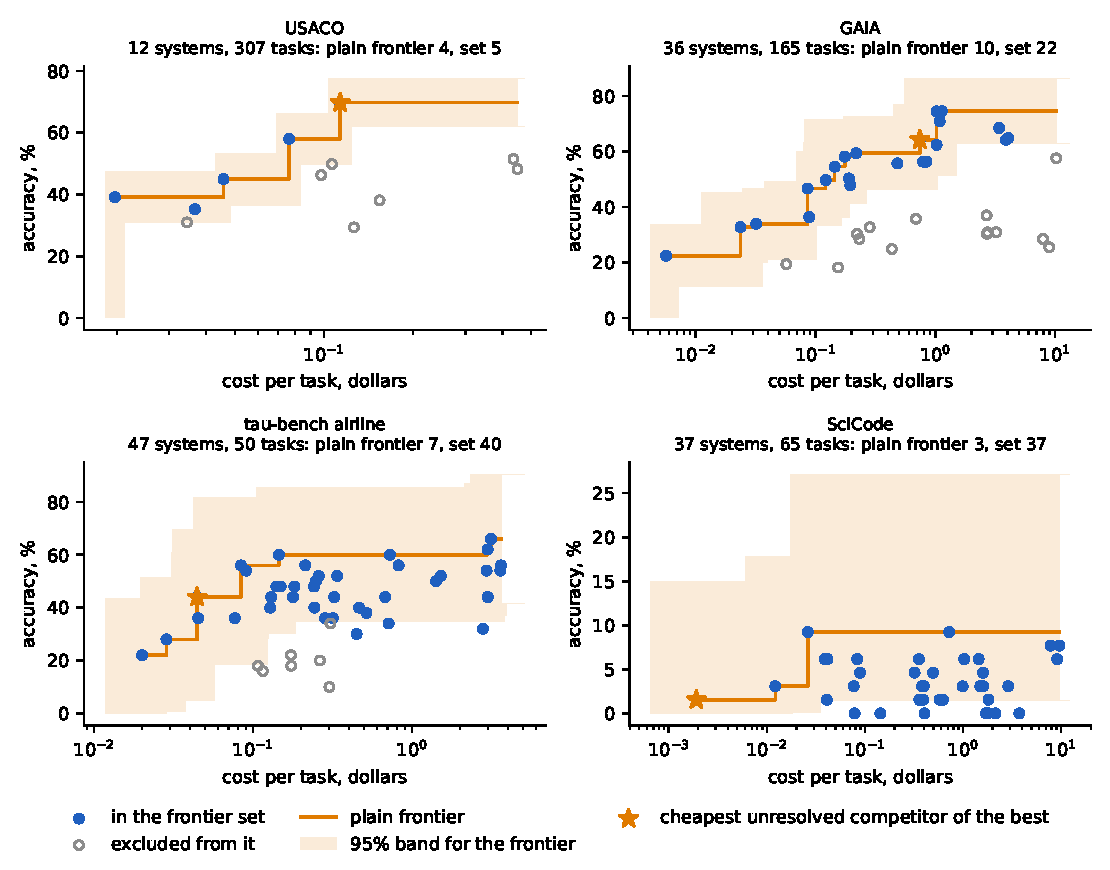
\includegraphics[width=\textwidth]{../figures/fig1_frontiers.pdf}
\caption{Cost per task against accuracy on each HAL benchmark. The orange staircase is the observed frontier. Filled points are systems that cannot be excluded from the frontier at the 5\% level; hollow points can be. The star is the cheapest plausible best: the cheapest system that cannot be excluded as the most accurate. Costs of zero are drawn at $10^{-4}$ dollars. The dagger marks the board whose costs are run totals spread over the tasks and treated as fixed.}
\label{fig:frontiers}
\end{figure}

\begin{figure}[t]
\centering
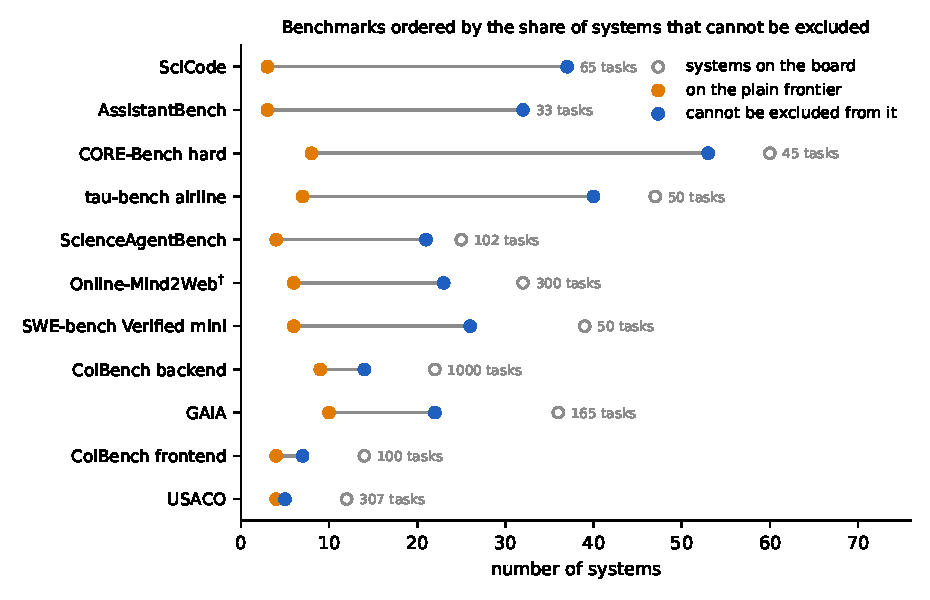
\includegraphics[width=0.7\textwidth]{../figures/fig2_setsizes.pdf}
\caption{For each benchmark, the number of systems on the plain frontier (orange), the number that cannot be excluded from it at the 5\% level (blue), and the number of systems on the board (hollow), with the task count beside it. Benchmarks are ordered by the share of their systems that cannot be excluded.}
\label{fig:setsizes}
\end{figure}

Table~\ref{tab:hal} and Figures~\ref{fig:frontiers} and~\ref{fig:setsizes} give the audit. Four readings.

\paragraph{The frontier is far less certain than the picture suggests.}
Across the \NumHalBoards{} benchmarks \NumHalObservedFrontier{} of \NumHalSystems{} systems sit on the observed frontier, but \NumHalFrontierSet{} cannot be excluded from it. The simultaneous margin is \NumHalMarginSeMin{} to \NumHalMarginSeMax{} standard errors of a paired difference, and on a board of 50 tasks a paired standard error is several accuracy points, so a system is ruled off the frontier only when a cheaper one leads it by ten to fifteen points.

\paragraph{Task count decides what can be said.}
The two boards where the set nearly equals the observed frontier are USACO (\NumUsacoTasks{} tasks: frontier \NumUsacoFrontier, set \NumUsacoSet) and ColBench backend programming (\NumColbenchBackendProgrammingTasks{} tasks: frontier \NumColbenchBackendProgrammingFrontier, set \NumColbenchBackendProgrammingSet). The two boards where nothing can be excluded are AssistantBench (\NumAssistantbenchTasks{} tasks, accuracies up to \NumAssistantbenchTopAcc\%) and SciCode (\NumScicodeTasks{} tasks, up to \NumScicodeTopAcc\%): with success rates that low and samples that small, no cheaper system can be shown to beat any other. CORE-Bench hard, with \NumCorebenchHardSystems{} systems on \NumCorebenchHardTasks{} tasks, keeps \NumCorebenchHardSet{} of them in the set.

\paragraph{The best is often clear even when the frontier is not.}
The best set is a single system on \NumHalBoardsBestOne{} boards (\NumHalBoardsBestOneNames) while the frontier set on those boards is larger. This is by construction: a system's rivals for the best set are all the other systems, and for the frontier set only the cheaper ones, with nearly the same margin, so the frontier set contains the best set, and a cheap, weak system stays in it whenever no cheaper system beats it by the margin. The frontier set is a statement about every system's own neighbourhood of cheaper rivals, and on most boards those neighbourhoods are thinly measured.

\paragraph{The cheapest plausible best is usually not the top system.}
On \NumHalBoardsCheaperBestInformative{} of \NumHalBoards{} boards the cheapest system that cannot be told apart from the best is a different and cheaper system than the most accurate one; on \NumHalBoardsBestAll{} further boards (\NumHalBoardsSetAllNames) the best set is the whole board, so the cheapest plausible best is simply the cheapest system and the statement is empty. The gaps are large: on tau-bench airline the top system costs \$\NumTaubenchAirlineTopCost{} per task and scores \NumTaubenchAirlineTopAcc\%, while the cheapest plausible best costs \$\NumTaubenchAirlineCbCost{} and scores \NumTaubenchAirlineCbAcc\%; on GAIA the pair is \$\NumGaiaTopCost{} at \NumGaiaTopAcc\% against \$\NumGaiaCbCost{} at \NumGaiaCbAcc\%; on SWE-bench Verified mini, \$\NumSwebenchVerifiedMiniTopCost{} at \NumSwebenchVerifiedMiniTopAcc\% against \$\NumSwebenchVerifiedMiniCbCost{} at \NumSwebenchVerifiedMiniCbAcc\%. A reader should not take this as "the cheap system is as good"; it says that \NumTaubenchAirlineTasks{} tasks cannot show that it is worse, at a level that accounts for all \NumTaubenchAirlineSystems{} systems being compared at once. The right response is more tasks, not a cheaper purchase.

\paragraph{The frontier winner's curse on HAL.}
\begin{table}[t]
\centering\small
\resizebox{\textwidth}{!}{\begin{tabular}{lrrrrrr}
\toprule
 & & & \multicolumn{2}{c}{Shrinkage, iterated bootstrap (pt)} & Shrinkage, conditional (pt) & Below strongest \\
Benchmark & On frontier & With a cheaper rival & mean & max & mean & cheaper rival after adjustment \\
\midrule
assistantbench & 3 & 2 & 3.3 & 5.3 & 1.1 & 1 \\
colbench backend programming & 9 & 8 & 0.3 & 0.5 & 0.1 & 0 \\
colbench frontend design & 4 & 3 & 0.2 & 0.5 & 0.4 & 1 \\
corebench hard & 8 & 7 & 4.3 & 7.7 & 3.5 & 4 \\
gaia & 10 & 9 & 1.2 & 2.4 & 1.3 & 2 \\
online mind2web$^{\dagger}$ & 6 & 5 & 0.6 & 0.9 & 0.1 & 0 \\
scicode & 3 & 2 & 0.2 & 0.5 & 0.1 & 0 \\
scienceagentbench & 4 & 3 & 0.8 & 1.6 & 0.1 & 0 \\
swebench verified mini & 6 & 5 & 1.0 & 2.3 & 0.1 & 0 \\
taubench airline & 7 & 6 & 4.4 & 9.4 & 2.8 & 3 \\
usaco & 4 & 3 & 0.0 & 0.1 & 0.0 & 0 \\
\midrule
All & 64 & 53 & 1.7 & 9.4 & 1.1 & 11 \\
\bottomrule
\end{tabular}
}
\caption{Selection-adjusted accuracy of the systems on HAL's observed frontiers. Shrinkage: reported accuracy minus the adjusted estimate, in points, over the frontier members that have a cheaper rival. The last column counts frontier members whose iterated-bootstrap estimate falls below the reported accuracy of their strongest cheaper rival. Every member is listed in the supplement.}
\label{tab:cursehal}
\end{table}
Table~\ref{tab:cursehal} applies the corrections to the \NumCurseMembers{} systems on HAL's observed frontiers, \NumCurseWithRival{} of which have a cheaper rival. The iterated bootstrap takes \NumCurseMeanShrinkPt{} points off a frontier member's reported accuracy on average and \NumCurseMaxShrinkPt{} at most; the conditional estimate takes \NumCurseMeanShrinkCondPt{} on average. For \NumCurseBelowRival{} of the \NumCurseMembers{} members, on \NumCurseBoardsBelow{} boards, the adjusted accuracy falls below the reported accuracy of the strongest cheaper rival: at its adjusted accuracy the system would not be on the frontier at all. The corrections are largest where the tasks are few and the frontier members many, CORE-Bench hard and tau-bench airline, and negligible on USACO and ColBench backend, where the tasks are many.

\paragraph{Certifying entrants on HAL's own timeline.}
\begin{table}[t]
\centering\small
\resizebox{\textwidth}{!}{\begin{tabular}{lrrrrrrr}
\toprule
 & & & & & \multicolumn{3}{c}{Certified} \\
Benchmark & Systems & Cheapest so far & Entrants & Dominated & unadjusted & spending & fallback \\
\midrule
assistantbench & 32 & 2 & 1 & 29 & 0 & 0 & 0 \\
colbench backend programming & 22 & 3 & 7 & 12 & 3 & 2 & 3 \\
colbench frontend design & 14 & 3 & 1 & 10 & 0 & 0 & 0 \\
corebench hard & 60 & 6 & 12 & 42 & 1 & 0 & 0 \\
gaia & 36 & 5 & 11 & 20 & 1 & 0 & 0 \\
online mind2web$^{\dagger}$ & 32 & 6 & 10 & 16 & 1 & 1 & 1 \\
scicode & 37 & 4 & 0 & 33 & 0 & 0 & 0 \\
scienceagentbench & 25 & 3 & 5 & 17 & 0 & 0 & 0 \\
swebench verified mini & 39 & 5 & 10 & 24 & 2 & 1 & 1 \\
taubench airline & 47 & 5 & 7 & 35 & 1 & 0 & 0 \\
usaco & 12 & 1 & 5 & 6 & 3 & 2 & 2 \\
\midrule
All & 356 & 43 & 69 & 244 & 12 & 6 & 7 \\
\bottomrule
\end{tabular}
}
\caption{Frontier entrants on each HAL board, walking the submissions in date order with each system's mean cost per task fixed on arrival. Cheapest so far: the system was cheaper than everything before it and joined the frontier with no rival to beat (no test). Entrants: the system beat every cheaper system on arrival and was tested against the most accurate of them with the selective record test and the per-date factor. Dominated: a cheaper earlier system was at least as accurate, so the system was never on the frontier. Certified: at the 5\% level with only the per-date factor applied (unadjusted), under alpha-spending, and under the online fallback, the levels being spent per date with an entrant; the last two control the family-wise error over the board's whole chain.}
\label{tab:certify}
\end{table}
Table~\ref{tab:certify} applies the rule of Section~\ref{sec:certify} to each board's history. Of \NumCertSystems{} arrivals, \NumCertCheapest{} were the cheapest system so far and joined the frontier without a rival to beat, \NumCertDominated{} were dominated on arrival by a cheaper system and were never on it, and \NumCertEntrants{} (\NumCertEntrantsPct\%) beat every cheaper system and were frontier entrants in the sense a leaderboard would announce. Tested against their most accurate cheaper rival, \NumCertUnadjusted{} of the \NumCertEntrants{} pass at the 5\% level with only the per-date factor applied, and \NumCertSpending{} under alpha-spending and \NumCertFallback{} under the online fallback, the levels being spent over the \NumCertDatesWithEntrants{} dates on which an entrant arrived. The certified steps are the large, well-measured ones, \NumCertMinMarginPt{} to \NumCertMaxMarginPt{} points on boards with at least \NumCertMinTasks{} tasks. The rest are of three kinds. \NumCertSmallStepSmallBoard{} entrants beat their rival by under five points on boards of at most 165 tasks, where such a step is within about one standard error. \NumCertMultiDate{} of the \NumCertEntrants{} entrants arrived on a date with other submissions, so that the best-of-date selection is priced by the per-date factor. And \NumCertBudgetExhausted{} entrants pass the 5\% level after the per-date factor but not the level left in the alpha-spending budget by the time they arrive, which is the price of controlling the error over the whole chain, as the companion paper found on its boards. A maintainer who announced every entrant as "new on the frontier" would have made \NumCertEntrants{} claims, of which \NumCertSpending{} to \NumCertFallback{} survive a guarantee, depending on the rule.

\section{Limitations}
\label{sec:limits}
Tasks are treated as exchangeable draws. Where tasks cluster (several from one repository, one website, one problem family) the standard errors are optimistic, as in any task-level analysis, and a cluster bootstrap would widen the margins. Each system has one run; run-to-run randomness of the same system on the same task is not in the standard errors, and HAL does not provide repeated runs. Costs depend on prices, which change; we fix one table and say which, and a reader pricing a run under another table should rebuild the frontier rather than reuse ours. Systems may have been tuned on the public tasks, which inflates every accuracy on the board and is outside the model. Outcomes are taken as HAL recorded them; HAL has since disclosed that on tau-bench airline its Generalist agent's episodes that never terminated were recorded as failures, so those rows are lower bounds on that scaffold's accuracy \citep{liu2026halissues}. The retention guarantee is asymptotic and per system; the joint guarantee is only simulated. On Online-Mind2Web the cost is a run total treated as fixed. The set uses one margin for the whole board, which is conservative when the systems are many; per-system margins would give a smaller valid set. Finally, the set is a statement about $K$ specific systems on $T$ specific tasks, and a new system or a new task changes it.

\section{Recommendations}
\begin{enumerate}
\item Report the frontier set beside the frontier. A board that draws a frontier from point estimates should say which systems cannot be excluded from it, at a stated level, and how many tasks that statement rests on.
\item Publish per-task costs. The confidence set needs them to carry the cost uncertainty, and the audit shows that run totals alone can hide a fourfold difference in price between two dates.
\item Price every run under one table and name the table and its date.
\item Give buyers the cheapest plausible best, with its level, rather than the top system.
\item Certify frontier entrants with the record test against the most accurate cheaper system, with costs fixed on arrival and an error budget spent over the calendar.
\end{enumerate}

\section{Conclusion}
A cost-accuracy frontier is an estimate. Treated as one, with a confidence set in place of a line, HAL's benchmarks say less than the lines suggest and more than nothing: on some boards the frontier is sharp, on most it is wide, and on a few it is empty of content until more tasks are run. The tools here let a maintainer say which, and let a new system be placed on the frontier with a guarantee that survives its own selection.

\section*{Reproducibility}
Code, the compact per-task records derived from HAL's public traces, the simulation and the audit are in the paper's repository; the methods are in the open-source package \texttt{honestboard} (module \texttt{frontier}). Raw HAL archives are not redistributed.

\bibliographystyle{plainnat}
\bibliography{refs}
\end{document}
